\section{Überblick über Neural Networks}
In den letzten Jahren hat die Technik der Neuronalen Netzwerke erneut stark an Popularität gewonnen. Dies liegt zum einen an der gestiegenen verfügbaren Rechenleistung und zum anderen an der Entwicklung hierfür notwendiger Algorithmen.\\
Allgemein lassen sich diese Netze in zwei große Gruppen aufteilen: die der \textsc{Feed Forward Neural Networks} und die der \textsc{Recurrent Neural Networks}, welche im Folgenden als \textsc{FFNN} respektive \textsc{RNN} bezeichnet werden.\\

Ein \textsc{FFNN} besteht aus mehreren Ebenen, welche jeweils aus verschiedenen nicht-linearen Einheiten (Neuronen) zusammengesetzt sind. Die erste dieser Ebenen wird zur Eingabe und die letzte zur Ausgabe eines Signals genutzt. Eine schematische Darstellung ist im linken Teil der Abbildung \ref{fig:ffnn_rnn_structure} zu finden. Die Einheiten zweier benachbarter Ebenen sind mit individuellen Gewichten vollständig in Richtung der Ausgabe verbunden. Dies bedeutet, dass jedes Neuron $x^n_i$ sein Signal an alle Neuronen der folgenden Ebene $x^{n+1}_j$ mit einem individuellen Gewicht $w^n_{i \rightarrow j}$ weitergibt. Zwischen den Einheiten innerhalb einer Ebene bestehen keinerlei Verbindungen.\\
Damit ein solches Netzwerk Vorhersagen treffen kann, müssen die Gewichte in einem Trainingsvorgang angepasst werden. Dies wurde durch die Entwicklung des \textsc{Backpropagation}-Algorithmus stark vereinfacht. Hierbei werden die Gewichte so angepasst, dass eine Kostenfunktion minimiert wird \cite[S. 225-290]{bishop}.\\

\begin{figure}[H]
    \centering
    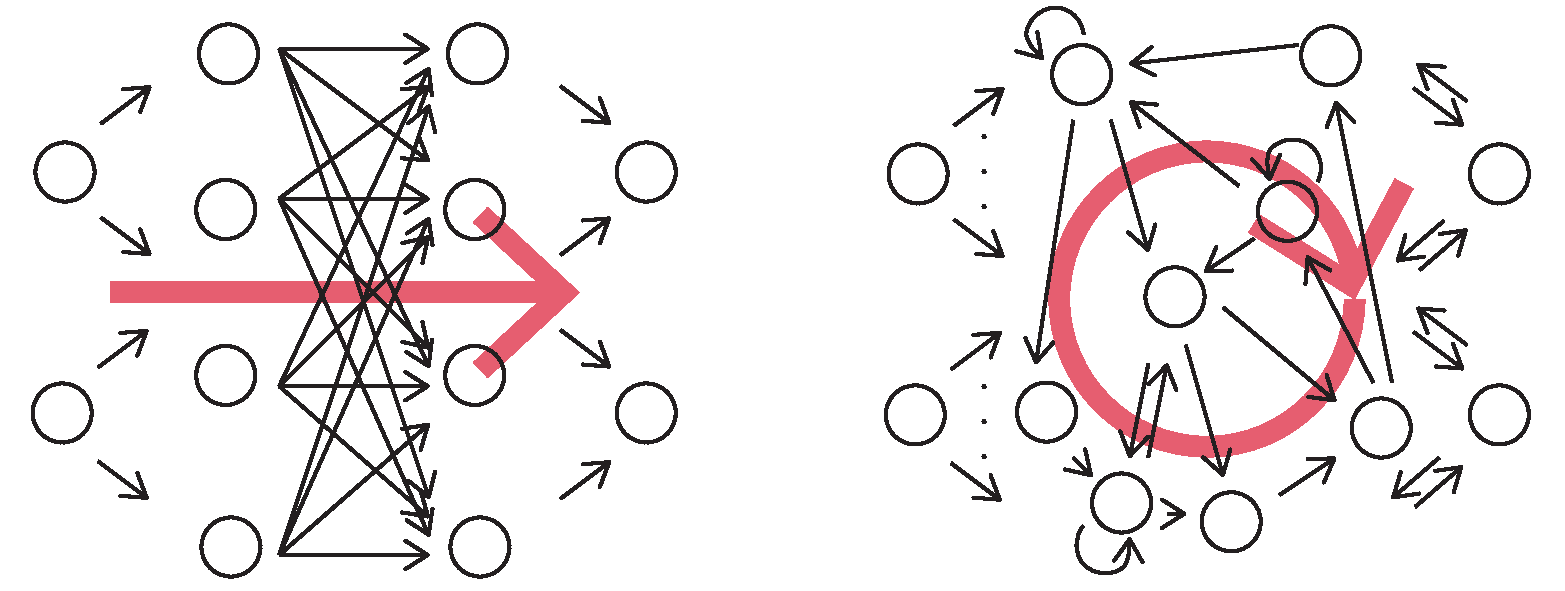
\includegraphics[width = 0.9 \textwidth]{figures/ffnn_rnn_structure(new).pdf}
    \caption{Schematische Darstellung eines \textsc{FFNN} mit vier Ebenen (links) und eines \textsc{RNN} (rechts) mit ihren jeweiligen Verbindungen und der Eingangs- und Ausgangsebene. Der Informationsfluss ist in rot eingetragen (nach \citep{jeagerTut2002}).}
    \label{fig:ffnn_rnn_structure}
\end{figure}

Ein \textsc{RNN} hat einen ähnlichen Aufbau, doch können hier alle Einheiten an alle anderen Einheiten Signale weitergeben und von diesen erhalten. Die schematische Struktur ist im rechten Teil der Abbildung \ref{fig:ffnn_rnn_structure} dargestellt. Dies kann die Vorhersage in bestimmten Anwendungsbeispielen wie der Text- und Sprachanalyse verbessern.\\
Ein Nachteil ist, dass zum Trainieren nicht mehr der einfachere \textsc{Backpropagation}-Algorithmus genutzt werden kann, sondern eine für \textsc{RNN}s abgewandelte Form genutzt werden muss. Für den prominenteste Algorithmus werden die verschiedenen Zustände die das \textsc{RNN} im Laufe der Signal-Propagation annimmt nacheinander betrachtet und auf diese zeitliche Entwicklung anschließend der \textsc{Backpropagation}-Algorithmus angewendet. Diese Methode ist unter dem Namen \textsc{Backpropagation through Time} (BTT) bekannt. Sie ist zum einen rechenaufwendiger und zum anderen auch instabiler, da das Verschwindenden und auch das Explodieren des Gradienten der Kostenfunktion deutlich wahrscheinlicher als bei der gewöhnlichen \textsc{Backpropagation} ist, wodurch der Trainingsvorgang instabil werden kann\citep{pascanu, jeagerTut2002}.
